\documentclass[conference]{IEEEtran}


\usepackage[dvips]{graphicx}
\usepackage{amsmath,amssymb}
\usepackage{algorithm}
\usepackage{algorithmic}
\usepackage{flushend}

%added by mohsin
\usepackage[usenames, dvipsnames]{color}
\usepackage{tikz}

\usepackage{url}

%\usepackage[
%backend=biber,
%style=numeric,
%sorting=ynt
%]{biblatex}
 
%\addbibresource{ref.bib}


%newcommand added by mohsin
\newcommand{\asymcloud}[2][.1]{%
\begin{scope}[#2]
\pgftransformscale{#1}%    
\pgfpathmoveto{\pgfpoint{261 pt}{115 pt}} 
  \pgfpathcurveto{\pgfqpoint{70 pt}{107 pt}}
                 {\pgfqpoint{137 pt}{291 pt}}
                 {\pgfqpoint{260 pt}{273 pt}} 
  \pgfpathcurveto{\pgfqpoint{78 pt}{382 pt}}
                 {\pgfqpoint{381 pt}{445 pt}}
                 {\pgfqpoint{412 pt}{410 pt}}
  \pgfpathcurveto{\pgfqpoint{577 pt}{587 pt}}
                 {\pgfqpoint{698 pt}{488 pt}}
                 {\pgfqpoint{685 pt}{366 pt}}
  \pgfpathcurveto{\pgfqpoint{840 pt}{192 pt}}
                 {\pgfqpoint{610 pt}{157 pt}}
                 {\pgfqpoint{610 pt}{157 pt}}
  \pgfpathcurveto{\pgfqpoint{531 pt}{39 pt}}
                 {\pgfqpoint{298 pt}{51 pt}}
                 {\pgfqpoint{261 pt}{115 pt}}
\pgfusepath{fill,stroke}         
\end{scope}}  

\begin{document}
\title{IMSI-based Routing and Identity Privacy in 5G}
\date{}%date stay empty

\author{
\IEEEauthorblockN{Mohsin Khan, Valtteri Niemi}
\IEEEauthorblockA{University of Helsinki and \\ Helsinki Institute for Information Technology \\ Helsinki, Finland \\ {mohsin.khan, valtteri.niemi}@helsinki.fi\\}
\and
\IEEEauthorblockN{Philip Ginzboorg}
\IEEEauthorblockA{Huawei Technologies and \\ Aalto University \\ Finland \\ philip.ginzboorg@huawei.com\\}}
\maketitle

\begin{abstract}
In 5G, identity privacy of a user is proposed to be protected by concealing the identifier of the user. In order to route the concealed identifier to the appropriate destination, certain information about the international mobile subscriber identity (IMSI) - country code and network code, need to be revealed. But, as was recently pointed out, the routing of requests for authentication information between visited and home network and also within the home network, needs more information about the IMSI to be revealed. Recently it was also revealed that the serving network needs to be able to identify a user with IMSI without relying on the home network for lawful interception purposes. In this new context, we re-examine published alternative solutions of identity privacy. We find the previously promising solutions e.g., solution based on public key of home network become less promising. We find the solution based on identity based encryption becomes more promising than it was before.
\end{abstract}

\section{Introduction} \label{intro}
In a mobile computing environment, the privacy of a user's current physical location is desirable \cite{Asokan_anonimity_1994,Varadharajan_anonimity_1997}. This is because lack of the location privacy enables third parties to track a user. To achieve location privacy, we need the privacy of the users' identities. In the 3GPP-defined mobile networks, a user has many identities, e.g., international mobile subscriber identity (IMSI), international mobile equipment identity (IMEI), mobile station international subscriber directory number (MSISDN), and many more. Privacy of all of these identities need to be protected. Among all of these identities, IMSI is the most difficult to protect. This is because IMSI is used for the identification of a user that is unknown (e.g., when connecting for the first time) to the network \cite{TS33401_inital_identification}, hence have no confidentiality protection. Serious effort has been put to solve this problem by the academic and 3GPP community. However, IMSI privacy is still not achieved, the so called IMSI catchers are still in existence \cite{catch_me_if_you_can, IMSI_Catcher_Adrian_2016, pets2017} and have become very cheap (in the order of hundreds of Euros) off-the-shelf \cite{IMSI_catcher_femtocell,Practical_attack_Altaf_shaik} technology. The alarming news is that the IMSI catchers are no more only an idle threat but have become a reality to the extent of mass surveillance \cite{washingtonpost2014}.

Identity privacy is a major requirement in 5G \cite{TS33501}. Many solutions have been proposed to defeat IMSI catchers \cite{TR33899}. Most of the solutions are based on some cryptographic techniques. Comparative analysis between the competitive solutions have been published \cite{ICTJournal}. There are pros and cons in every solution. 3GPP community is now at the verge of finalizing the specification for the first phase of 5G technology. A solution based on public key cryptography has been chosen to protect the privacy of IMSI \cite{TS33501} (in Section 6.12.2). In this solution, the home network (HN) owns the public-private key pair. The user equipment (UE) shall generate a concealed identity with the raw public key that was securely provisioned to the user in control of the HN. We call this solution as root-key based solution. 

An issue about routing authentication information has surfaced recently \cite{SUCIRouting}. We will explain this issue in Section \ref{section:IMSI-based-routing}. To solve this issue, the root-key based solution needs to reveal more information about the identity of a user. This reduces the effectiveness of root-key based solution. Another issue around lawful interception (LI) has been noticed recently \cite{SUCIRouting}. We will explain the issue in Section \ref{section:LI}. In Section \ref{section:categories}, we categorize the promising solutions based on the cryptographic techniques used. In Section \ref{section:comparison}, we will present a comparative analysis of the alternative categories of solutions in the light of these two new concerns as well as the relevant old concerns \cite{ICTJournal, IBE_mohsin}. We will see that the balance of pros and cons between different solutions changes significantly. The root-key based solution which appeared to be quite straightforward and effective solution \cite{ICTJournal} becomes less effective and requires more implementation effort. On the other hand, a solution based on identity based encryption (IBE) \cite{ICTJournal,IBE_mohsin} which had its own cons, solves both of the concerns of IMSI-based routing and LI. In this light we will argue that solution based on identity based encryption could be the most effective and also fairly straightforward solution to protect the privacy of IMSI.

In order to present a smooth discussion, we need to first explain some background. We will present an abstract view of a mobile network. This view is abstract enough to cover both LTE and 5G, even earlier generations. We will discuss how IMSI is used, how privacy of IMSI is vulnerable in the legacy networks. We will also discuss the principles of different categories of solutions very briefly. 

\section{Background} \label{background}
\subsubsection{IMSI}
A unique International Mobile Subscriber Identity (IMSI) shall be allocated to each mobile subscriber in the GSM/UMTS/EPS system \cite{TS23003}. An IMSI is usually presented as a $15$ digit number but can be shorter. The first $3$ digits are the mobile country code (MCC), which are followed by the mobile network code (MNC), either $2$ or $3$ digits. The length of the MNC depends on the value of the MCC. The remaining digits are the mobile subscription identification number (MSIN) within the network's customer base \cite{TS23003}. 

In the legacy networks -- e.g., LTE, when a user equipment (UE) tries to connect to a network for the first time, the UE has to identify itself using IMSI \cite{TS33401_inital_identification}. Once the UE is identified, an authentication protocol (e.g., EPS AKA \cite{TS33401_inital_identification}) is run in between the UE and the network. If the authentication protocol runs successfully, the network serves the UE with the services the UE is authorized to avail.


\subsubsection{Mobile Network}
A mobile network consists of UE, serving network (SN) and HN. Both of the SN and HN consist of radio access network (RAN) and core network (CN). The RAN of SN provides the connectivity in between UE and CN of SN. On the other hand, the CN of SN connects itself with the CN of HN via IPX. Note that in a non-roaming situation, the SN and HN are the same network. See Figure \ref{fig:security_architecture_abstraction}.

\subsubsection{IMSI Catchers}
There are two more entities which are not part of the network but relevant in our discussion, because they attack the network. They are passive IMSI catchers and active IMSI catchers \cite{IBE_mohsin}. The interface UE-SN is a logical interface in between UE and SN. This interface is initially unprotected. The logical interface SN-HN between SN and HN is protected and the security of this interface is out of the scope of this paper. The passive IMSI catchers eavesdrop on the UE-RAN interface when it is unprotected to extract an IMSI. The active IMSI catchers impersonate a legitimate SN and run a legitimate-looking protocol with the UE in order to find out the IMSI. The HN and UE both know the IMSI and they are trusted. Both passive IMSI catchers and active IMSI catchers are untrusted. 

\subsubsection{Solutions Against IMSI catchers}
In legacy networks, the approach of protecting IMSI privacy is to use a temporary identifier instead of the actual IMSI and keep changing the temporary identifier at a feasible frequency. Note that the temporary identifier has to be assigned over a confidentiality protected channel and different entities of the network may assign different temporary identifiers to the UE. In the LTE network, the temporary identifier assigned by serving network (SN) is called globally unique temporary identity (GUTI) \cite{TS23003} and the home network (HN) does not assign any temporary identifier to the UE. However, during the initial attachment of a UE to the SN, the UE has neither a GUTI nor a security context with the SN that can assign it with a GUTI. Besides, GUTI can be lost by either one or both of the UE and the SN. This would force the UE to reveal its IMSI to the SN to keep itself from permanently locked out of the network. This problem gives an opportunity to an active IMSI catcher who impersonates a legitimate SN and forces the UE to run the initial attachment protocol. This also gives an opportunity to a passive IMSI catcher to eavesdrop the IMSI sent in clear text. To fight against these active IMSI catchers in 5G, different solutions \cite{pseudonym_valtteri_philip, pseudonym_ericsson, CCS15, SSR15, wisec17, pseudonym_mohsin, ICTJournal, IBE_mohsin} have been proposed.

\section{Categories of Solutions} \label{section:categories}
All the solutions that we are aware of to defeat IMSI catchers are based on cryptographic encryption techniques. In this section we will look into different categories of solutions. The categories are drawn based on different cryptographic encryption techniques.

\begin{figure}
\begin{center}

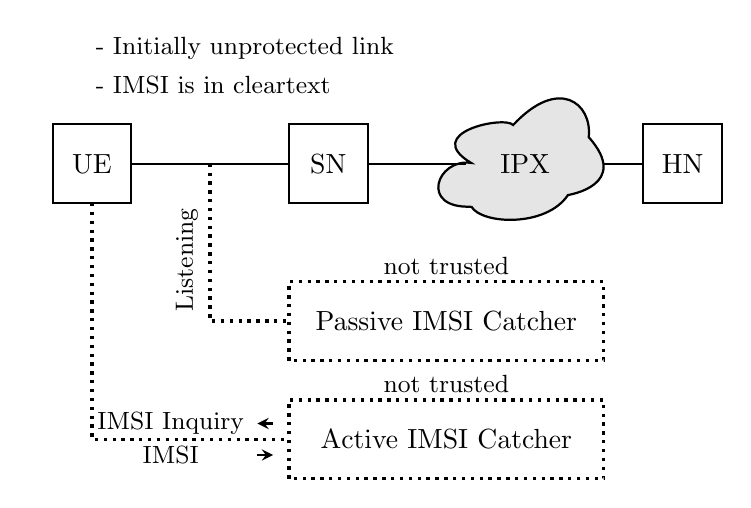
\begin{tikzpicture}

\draw[black, very thick, dotted] (3,-.5) rectangle (7,.5);
\draw node at (5 ,0) { Active IMSI Catcher };

\draw[black, very thick, dotted] (3,1) rectangle (7,2);
\draw node at (5 ,1.5) { Passive IMSI Catcher };


\draw[black, thick] (0,3) rectangle (1,4);
\draw node at (.5 ,3.5) { UE };


\draw[black, thick] (3,3) rectangle (4,4);
\draw node at (3.5 ,3.5) { SN };

\draw[black, thick] (1,3.5) -- (3,3.5);


\node (cloud) at (6,3.65) {\tikz \asymcloud{fill=gray!20,thick};};
\draw node at (6 ,3.5) { IPX };

\draw[black, thick] (4,3.5) -- (5.25,3.5);


\draw[black, thick] (7.5,3) rectangle (8.5,4);
\draw node at (8 ,3.5) { HN };

\draw[black, thick] (7.5,3.5) -- (7,3.5);


\draw[black,very thick, dotted] (.5,3) -- (.5,0) -- (3,0);
\draw[black,very thick, dotted] (2,3.5) -- (2,1.5) -- (3,1.5);

\draw node at (5 ,.7) { \small not trusted};
\draw node at (5 ,2.2) { \small not trusted};

\node[label={[label distance=0.5cm,text depth=-1ex,rotate=0,font=\small]right: - Initially unprotected link}] at (-.2,5.0) {};
\node[label={[label distance=0.5cm,text depth=-1ex,rotate=0,font=\small]right: - IMSI is in cleartext}] at (-.2,4.5) {};

\node[label={[label distance=0.5cm,text depth=-1ex,rotate=90,font=\small]right: Listening}] at (1.55,1) {};



\draw node at (1.5 ,.2) { \small IMSI Inquiry};
\draw node at (1.5 ,-.2) { \small IMSI};

\draw [->,>=stealth,thick] (2.8,.2) -- (2.6,.2);
\draw [->,>=stealth,thick] (2.6, -.2) -- (2.8,-.2);

%\draw [->,>=stealth,ultra thick] (2, 3.6) -- (2,4.1);

 
\end{tikzpicture}

\caption{High-level Security Architecture}
\label{fig:security_architecture_abstraction}       % Give a unique label
\end{center}
\end{figure}




%\begin{itemize}

\subsubsection{Pseudonym Based}
The pseudonym based solutions as proposed in \cite{pseudonym_ericsson,pseudonym_valtteri_philip,CCS15,SSR15,pseudonym_mohsin} fall in the category of symmetric key encryption.  In this kind of solutions, temporary identifiers called pseudonyms are assigned to a UE. Next time when the UE tries to identify itself to an SN, it uses a pseudonym instead of IMSI. Periodically, whenever there is an opportunity, the HN sends a new pseudonym to the UE with confidentiality and integrity protection using a symmetric key -- that is why it falls under the category of symmetric key encryption. One such opportunity is when the HN sends the authentication vector to an SN.

\subsubsection{Certificate based} In the certificate based encryption, the public key is signed by a trusted third party. The sender has to be pre-provisioned with the root certificate so that the sender can authenticate the public key of the receiver. Use of certificate based public-key encryption to conceal long-term identity has been suggested in 3GPP TR 33.821 \cite{TR33821}. The UE encrypts the IMSI using the public key of the SN before sending. To use certificate based public-key cryptography, we need to figure out who are the root certificate authorities (CA) and who else can be a CA, who owns a public key, how a certificate can be revoked, and how the UE can be re-provisioned with a new root certificate if needed. Different solutions can be devised based on the choice of root CAs and other CAs.


\subsubsection{Root-key Based} In the root-key based encryption, no runtime authentication of the public key is required, because a very limited number of public keys are used in the system and all the senders are pre-provisioned with all the existing public keys. Use of root-key has been proposed in 3GPP TR 33.899 in solution \#7.3. In this approach only one pair of public-private key pair exists. This key pair is owned by the HN and we call it the root-key. The HN provisions the public key to all its UEs.  Instead of sending the IMSI, the UE encrypts the IMSI with the public root key and sends the result to the SN along with MCC and MNC. The SN sends the encrypted IMSI to the HN. The HN decrypts the IMSI and sends the IMSI back to the SN along with an authentication vector (AV).

\subsubsection{Identity Based} In IBE, the public key of a receiver is computed from the identity of the receiver and the public key of a trusted third party known as private key generator (PKG). The public key of the trusted third party has to be provisioned to the sender. The private key of the receiver is computed as a function of the identity of the receiver and the private key of the PKG. The private key of the receiver has to be provisioned to the receiver by the PKG. In IBE based solution \cite{IBE_mohsin,ICTJournal}, the HN is the PKG. The HN has a public-private key pair. The UEs are provisioned with the public key of the HN. The SNs which have a roaming agreements with the HN are also provisioned with their respective private keys by the HN. When a UE identifies itself with IMSI, it encrypts the IMSI using the public key of the SN. The UE computes the public key of the SN as function of the identity of the SN and the public key of the HN. The most interesting aspect of this solution is that there is no certificate involved and the SN can decrypt the encrypted IMSI.
%\end{itemize}

All these solutions try to defeat the IMSI catchers by concealing the permnanent identity -- IMSI. The concealed identity is known as subscription concealed identifier (SUCI) and the permanent idenity is known as subscription permanent identifier (SUPI) \cite{TS33501}. In the next two sections we will explain the issues around IMSI-based routing and LI that impacts the effectiveness of different categories of solutions.

\section{IMSI-based Routing} \label{section:IMSI-based-routing}
First aspect of the issue is the routing of authentication information requests inside one mobile network. Subscribers' database of the mobile network operator is typically divided into several parts to increase lookup efficiency. In today's cellular systems, serving network's request for authentication information is routed to the correct database partition based on typically the first one to three digits of the MSIN \cite{S3180761}.

Subscribers' database in 5G system is called Unified Data Management (UDM), and similarly to the previous generations of cellular systems, there are likely to be several UDM entities in the mobile network (in order to increase lookup efficiency). 

If the MSIN in the authentication information request message is encrypted, then either, (i) MSIN has to be decrypted before routing, or (ii) the routing of the message to the correct UDM is based on another part in the message. The second of these options is more attractive than the first, because the decryption entity may become a new bottleneck in the 5G system. Therefore, 3GPP SA3 is moving towards option (ii). (One solution proposed  in 3GPP SA3 uses home network's public key identifier for routing purposes; another solution proposes leave required SUCI routing information unencrypted as part of the SUCI \cite{S3180763}.)

Another aspect of the issue is the routing of authentication information requests between different mobile networks. Mobile network operators interconnect their networks via IP exchanges (IPXs). Typically MCC and MNC are sufficient for routing visited network's requests for authentication information to the home network. But, if a mobile virtual network operator  (MVNO) has (i) the same MCC and MNC as the MNO from whom it purchases networking services in bulk; and (ii) subscribers' database in a completely different location from that of MNO, then knowing only MCC and MNC is not enough to identify the home network. In that case, an IPx uses part of MSIN, in addition to MCC and MNC, for routing visited network's requests to the home network.

All in all, authentication information requests in 5G system should include some cleartext routing information, in addition to MCC and MNC. Please note that this extra information may be used for tracking the user: for example, if information equivalent of four MSIN digits is revealed, then the probability of identifying a user becomes ten thousand times bigger. On the other hand, solutions in which the MSIN is decrypted at SN, e.g., IBE based solution do not have this weakness.


\section{Lawful Interception} \label{section:LI}
According to 3GPP specification \cite{TS33106}, LI requirement is: the SN should be able to identify a user with the IMSI without relying on the HN. However, if the SN can not decrypt the MSIN coming from the UE (because it may be encrypted by the public key of the home network or be a pseudonym known to HN only), then the SN has to learn the MSIN from the HN. This is the case for both the root-key based or pseudonym based solution. 

In root-key and pseudonym based solutions, the SN has to learn the IMSI from the HN. Apparently it means that the SN is relying on the HN to resolve the IMSI of a user. However, to be confident that the HN gave the original IMSI of a user, several ways have been proposed in 3GPP SA3 \cite{NokiaLI,NokiaLI1,EricssonLI,CATTLI,KPNDOCOMOLI}. In \cite{NokiaLI, NokiaLI1}, the SN receives the SUCI and a hash computed on the SUCI and SUPI from the UE. The SN also receives the SUPI from the HN. So the SN can compute the hash on SUCI and SUPI. If the HN gave a fake SUPI to the SN then the hash computed by the SN would not match with the hash the SN received from the UE. In \cite{EricssonLI}, the UE sends its SUPI to SN using the NAS security mode command procedure. Since NAS security mode command procedure is usually confidentiality protected, SUPI privacy is also protected. The SN does not provide service to UE, if SUPI indication from UE and HN do not match. In \cite{CATTLI}, the combination of NAS security mode command procedure and the hash based technique is used. The hash based technique is used when the NAS encryption is not active. All these solutions add overhead by adding new signalling messages or parameters to the messages of the authentication and key agreement or of NAS security mode command. However, the solution in \cite{KPNDOCOMOLI} vouch for binding SUPI in generating the anchor key in the VPLMN as mentioned in \cite{SUPIBinding}. So, if the HN gave a fake SUPI to the SN, the SN would generate a different key than that of the UE. Thus, the UE will not be able to get any service if the HN gives the SN a fake SUPI.


Nevertheless, the solutions in which MSIN can be decrypted in the SN do not have the concern of HN telling the truth or lie. This is because, the SN does not need the HN for resolving the MSIN -- the SN would learn the MSIN directly from the UE. This is the case for certificate based and IBE based solution. Unless the HN and the UE collude to fool the LI entity in the SN, the LI entity can trust that the identity given by the UE is correct after authentication of the UE has succeeded.


\section{Qualitative Comparison of Different Categories of Solutions} \label{section:comparison}
Qualitative comparison of different solutions based on different criteria was presented in \cite{ICTJournal,IBE_mohsin}. In this paper we take the same approach. For smoother reading, we present only those criteria which we have found to make a difference between solutions. We only compare according to the solution categories.  We have discussed two different categories of solutions: pseudonym based and public-key based. We have categorized the different public-key technologies into three categories: certificate based, root-key based and identity based. In Table \ref{table:comparison}, we present a comparison among the different solutions based on different criteria. We indicate the performance of the solutions based on each criteria according the following symbols : ++ very good, + good, +- somewhat okay, - not good.

\paragraph{Immunity Against Active IMSI Catchers} This is the most important criterion because the whole effort is to defeat the active IMSI catchers. Before the concern around IMSI-based routing surfaced, in pseudonym based and root-key based solution, it was sufficient to reveal MCC and MNC to route the SUCI to the appropriate destination. So, an active IMSI catcher could learn the MCC and MNC only. However, because of the concerns around IMSI-based routing, pseudonym based and root-key based solutions have to reveal more information from MSIN. It makes them less immune against active IMSI catchers. However, these solutions can still achieve certain degree of anonymity. So, we evaluate them with +-. Note that, in \cite{ICTJournal}, these two solutions were evaluated with +. The certificate based solution with global PKI can conceal even MCC and MNC. So, we evaluate them with ++. In IBE based solution, only MCC and MNC needs to be revealed. So we evaluate it with +.

\paragraph{Lawful Interception} \label{subsection:LI}
The LI requirement is that the SN should be able to identify a user with the IMSI without relying on the HN. Both in pseudonym based and root-key based solutions, the SN has to rely on the HN to identify a user with the IMSI -- HN sends the IMSI to the SN. To be confident that the HN gave the real IMSI some extra effort is required as mentioned in \cite{NokiaLI,NokiaLI1,EricssonLI,CATTLI,KPNDOCOMOLI}. Before the concern around LI surfaced, this extra effort was not required. Besides, in both of these solutions, it has to be assumed that the HN and UE are not colluding. Only under such assumption, the SN can trust that the IMSI given by the HN is correct. Since it needs the assumption, we evaluate these two solutions as +-. In certificate and IBE based solutions, the SUCI can be decrypted in the SN. So, these two categories of solutions do not have the concern of the HN telling the truth or lie. This is because, the SN does not need the HN for resolving the MSIN. The MSIN can be decrypted out of the SUCI by the SN itself. So, we evaluate both of these solutions with +.

\paragraph{Deployment and Maintenance Effort}
Pseudonym based approach does not require standardization. Changes in the SIM and HN -- operated by the same entity, is sufficient. So, it is relatively easy to deploy. However, it makes the subscription database very sensitive to any changes, hence the maintenance becomes difficult.  So, we rate this with +-. Certificate based solutions require setting up PKI and maintaining it. That is a lot of effort. So we rate certificate based solution with -. Root-key based and IBE based solutions are fairly easy to deploy and maintain. So we rate them with +.

\paragraph{Transparency to the Legacy SNs}
To enable the SN to identify a user with IMSI -- the LI requirement, the pseudonym based solutions require similar solutions as mentioned in \cite{NokiaLI,NokiaLI1,EricssonLI,CATTLI,KPNDOCOMOLI}. These solutions need the SN to understand extra message fields sent by the HN. This means the pseudonym based solutions are not transparent to the legacy SNs. However, pseudonym based solution would be transparent to the SNs if identifying a user using pseudonyms would become a sufficient LI requirement. So we evaluate them with +-. Consequently, even though previously it was a very important advantage of pseudonym based approach, it becomes a just okay solution now in this regard. So we rate this with +-. However, no other solutions are transparent to SNs. Because in all the other solutions, the SN has to receive ciphertext produced by public key -- none of the legacy SNs has to do that. So we rate all of them with -.

\paragraph{Signalling overhead}
In pseudonym based solution, the SN needs to know the IMSI of a user from the HN. To be confident that the IMSI given by the HN is correct, similar measures as mentioned in \cite{NokiaLI,NokiaLI1,EricssonLI,CATTLI,KPNDOCOMOLI} have to be implemented. This adds some extra signalling overhead on top of what exists in the legacy networks. However, pseudonym based solution does not use public key encryption. The use of only symmetric key encryption produces shorter ciphertext which keeps the signalling overhead significantly low. So we rate it with +.
Certificate based solutions require an extra round trip between the UE and the SN to exchange the certificate. This creates signalling overhead. Certificate based solution does not require the HN to give the IMSI to the SN. So, certificate based solution does not require the added signalling overhead as it requires in pseudonym based solution. This may sound that pseudonym based and certificate based solutions are equally good/bad in this criteria -- both of them need added signalling for different purposes. However, the added signalling overhead in pseudonym based solution is in the core network, whereas the added signalling overhead to exchange the certificates is in the radio network. Besides certificates can be quite long. So we rate certificate based solution with -. The root-key based solution requires the similar extra signalling as the pseudonym based solution requires. Besides it has to route the SUCI all the way to the HN. The SUCI is generated using public key encryption -- quite longer than pseudonyms. However, it does not need to exchange certificates -- a significant relieve. So we rate it with +-. IBE based solutions do not require any extra round trips or certificates -- less signalling overhead compared to certificate based solutions. IBE based solution does not require the HN to give the IMSI to the SN. For this reason, IBE based solution does not require the extra signalling overhead as the pseudonym based or root-key based solution require. However, IBE based solution produces SUCI which are quite longer than pseudonyms. So we rate them with +.

\paragraph{Computational overhead}
Pseudonym based solutions require some extra computation in the HN to generate next pseudonym of a user randomly. However, this is quite less complex in comparison with public key encryption. So, we rate it with ++. Certificate based solutions require to exchange and verify the certificate and compute public key encryption/decryption. This creates computational overhead. So, we rate it with -. However, both root-key and IBE based solutions require public key encryption and decryption but do not require verifying certificates. So we rate them with +.

\paragraph{Latency}
In pseudonym based solution, some extra signalling overhead is needed to add to enable the SN to serve the LI requirement. However, since pseudonym based solution uses symmetric key encryption and does not use public key encryption, the signalling and computational overhead is comparatively low. However, when the user is roaming, to resolve the IMSI, the pseudonym has to travel all the way to the HN -- increases latency. So we rate it with -. Certificate based solutions require an extra round trip between the UE and SN to exchange and verify the certificates, computes public key encryption and have longer message length. All these affect the latency. So we rate certificate based solution too with -. In the root-key based solution, when the user is roaming, to resolve the IMSI, the pseudonym has to travel all the way to the HN -- increases latency. So we evaluate it with -. The IBE based solutions do not require any extra round trips or certificates. However, they compute public key encryption and have longer message length. Hence the latency is affected. However, So we rate them with +-.


\paragraph{Key revocation}
Pseudonym based solution is a symmetric-key based solution. So it does not require any key revocation. So, we rate it with ++. However, all the public key based solutions require a mechanism of key revocation. In certificate based solution, to access the revocation list, a user has to connect to an SN. How a UE may know that the public key of the SN has already been revoked? On the other hand, in IBE based solutions, revocation is inherently complicated. One solution around this is to use short expiry time for the public keys of the SNs. By doing so, key revocation increases some overhead. So we rate both of them with -. In root key based solution no revocation is required because there is only one public key. If the corresponding private key is compromised, the UE has to be re-provisioned with the new public key. So we rate it with +.

\paragraph{Maturity}
We also look at the solutions from the point of view of the maturity of the technology. Use of pseudonyms for privacy purpose is not yet a very matured technology. Use of IBE is not yet widespread. So we rate both of them with -. However, certificate based public-key encryption technology is widespread and matured. Use of root-key can be viewed as a special case of certificate based public-key. So, we rate both of certificate based and root-key based solutions with +.

\paragraph{Mutual authentication} It is possible that in future there might be a need of mutual authentication between the UE and the SN without the intervention of the HN. In this respect we notice that pseudonym based and root-key based solution can not be used for mutual authentication. This is because, in these cases the IMSI is not visible to the SN without consulting with the HN. So, we rate these two categories with -. However, Certificate based and IBE based solutions can be extended into a mutual authentication protocol between UE and SN. One example can be found in \cite{ICTJournal}. So, we rate both of these two categories with +.
   

\paragraph{Summary of the Comparison}
Looking at the table, it seems evident that IBE based solution is the most promising solution. Certificate based approach is good in preventing active IMSI catchers and handling the requirement of lawful interception. But the solution is costly in almost all other aspects. Maybe, the industry is not yet ready to spend such expenses to provide user identity privacy. Even though pseudonym based approach is inexpensive from almost all the aspects, it becomes a bit less effective to achieve its original purpose - immunity against active IMSI catchers. Because of the LI issues, it also loses its most important merit - transparency with legacy SNs. The root-key based approach is also a bit less effective in serving its original purpose - immunity against active IMSI catchers. It also makes the lawful interception a bit more complicated than that of IBE based solution. However, key revocation in IBE may have some latency whereas no key revocation is required in root-key. But still, considering the effectiveness of the solution, we would like to conclude that IBE based solution is a better choice than the root-key based solution.


\begin{table*}
\begin{normalsize}
\begin{center}
\caption{Comparative evaluation of the solutions}
\begin{tabular}[t]{|l|c|c|c|c|}
\hline
%\multicolumn{1}{|c|}{} & \multicolumn{1}{|c|}{} & \multicolumn{7}{|c|}{\textbf{Public-key based Solutions}}\\
%\cline{3-9}
\multicolumn{1}{|c|}{\textbf{Criteria}} & \multicolumn{1}{|c|}{\textbf{Pseudonym}} & \multicolumn{1}{|c|}{\textbf{Certificate based}} & \multicolumn{1}{|c|}{\textbf{Root-key}} & \multicolumn{1}{|c|}{\textbf{IBE based}}\\
%\cline{3-5} \cline{7-9}
%\textbf{} &  & \textbf{V1} & \textbf{V2} & \textbf{V3} & \textbf{} & \textbf{JPL} & \textbf{PEMMA} & \textbf{PEFMA}\\
\hline \hline
Immunity to Active IMSI Catchers & +- & ++ & +- & + \\ \hline
Lawful interception & +- & + & +- & +  \\ \hline
Deployment and Maintenance Effort & +- & - & + & + \\ \hline
Transparency to the Legacy SNs & +- & - & - & - \\ \hline
Signalling overhead & + & - & +- & + \\ \hline
Computational overhead & ++ & - & + & + \\ \hline
Latency & - & - & - & +- \\ \hline
Key revocation & ++ & - & + & - \\ \hline
Maturity  & - & + & + & - \\ \hline
Mutual Authentication & - & + & - & + \\ \hline
\end{tabular}
\label{table:comparison}
\end{center}
\end{normalsize}
\end{table*}


\section{Conclusion}
User identity privacy in 3GPP  Release 15 -- the first release of 5G system, will be based on what we call a "root-key" solution. It impacts IMSI-based routing of messages and the legal interception (LI) entities in cellular networks.  We have analyzed these and other impacts for several solution types for user identity privacy. It was found that IBE based solution is in several ways better than the root-key based solution. In conclusion, IBE based solution for user identity privacy could be proposed for future 3GPP releases of 5G system.



%\section*{Acknowledgment}


\bibliographystyle{acm}
\bibliography{ref}{}


%\begin{thebibliography}{6}

%\bibitem{Cover}
%\textit{(Example for books)} T.M.Cover and J.A. Thomas, \emph{Elements of Information Theory}. New York: Wiley, 1991.

%\bibitem{Dobrushin}
%\textit{(Example for articles)} R.L. Dobrushin, ``Optimum information transmission through a channel with unknown parameters'',  \emph{Radiotech.Electron.}, vol.4, Dec.1959, pp. 1951-1956.

%\bibitem{Blachman}
%\textit{(Example for articles)} N.M. Blachman, ``Communication as a game'', \emph{in Proc. WESCON Conf.}, Aug. 1957, pp. 61-66.

%\bibitem{IEEE}
%\textit{(Example for web-links)} IEEE official website, Manuscript Templates for Conference Proceedings, Web: http://www.ieee.org/conferences\_events/conferences/publishing/templates.\newline html.

%\bibitem{Elissa}
%\textit{(Example for unpublished references)} K. Elissa, ``Title of paper if known'', unpublished.

%\bibitem{Nicole}
%\textit{(Example for references have been accepted for publication)} R. Nicole, ``Title of paper with only first word capitalized'', J. Name Stand. Abbrev., in press.

%\end{thebibliography}

%\printbibliography

\end{document}
